\SS\section{Case Studies} % We are studying multiple cases!
\label{s:case-studyAll}
To perform compelling case studies, we used our system on several examples, including one designed to be a worst case scenario for our approach. We also replicate many examples originally proposed by other papers, so that 
not all the code examples come from us. 

\subsection{An interactive GUI}
\label{s:case-study}
We start by presenting our GUI example; a program that interacts with the real world using I/O.
It demonstrates how to verify invariants over cyclic mutable object graphs.
Our example is particularly relevant since, as with most GUI frameworks, it uses the \emph{composite} programming pattern; arguably one of the most fundamental patterns in OO.

%Here we discuss how to use conventional OO programming patterns to take advantage of our system. Using those
%patterns allows to circumvent some of the apparent limitations of our system.
% At first glance it would seem that by only being able to validate immutable and encapsulated state one could not create validated classes with complicated, mutable interconnected object graphs.
%We show that this is not the case by encoding
%Our invariant is that everything in every movable container (and the top level component) should 
%-be inside the container 
%-not overlap with anyhing else inside
%Our containers represent boxes that completley contain other non-overlapping boxes.
Our case study involves a GUI with containers (\Q@SafeMovable@s) and \Q@Button@s.
The \Q@SafeMovable@ class has an invariant to ensure that its children are graphically contained within it and do not overlap. The \Q@Button@s move their \Q@SafeMovable@ when pressed. We have a \Q@Widget@ interface, which provides methods to get \Q!Widget!s' size and position as well as children (a list of \Q@Widget@s). Both \Q@SafeMovable@s and \Q@Button@s implement \Q@Widget@. Crucially, since the children of \Q@SafeMovable@ are stored in a list of \Q@Widget@s it can contain other \Q@SafeMovable@s, and all queries to their size and position are dynamically dispatched. Such queries are also used in \Q@SafeMovable@'s invariant.
Here we show a simplified version\footnote{The full version, written in L42, which uses a different syntax, is available in our artifact at \url{http://l42.is/InvariantArtifact.zip}}, where  \Q@SafeMovable@ has just one \Q@Button@ and certain sizes and positions are fixed. Note that \Q@Widgets@ is a class representing a mutable list of \Q@mut@ \Q@Widget@s.
\begin{lstlisting}
class SafeMovable implements Widget {
  rep Box box; Int width = 300; Int height = 300;

  @Override read method Int left() { return this.box.l; }
  @Override read method Int top() { return this.box.t; }
  @Override read method Int width() { return this.width; }
  @Override read method Int height() { return this.height; }
  @Override read method read Widgets children() { return this.box.c; }
  @Override mut method Void dispatch(Event e) {
    for (Widget w:this.box.c) { w.dispatch(e); }}
  read method Bool invariant() {../* presented later */..}
  SafeMovable(capsule Widgets c) { this.box = makeBox(c); }
  static method capsule Box makeBox(capsule Widgets c) {
    mut Box b = new Box(5, 5, c);
    b.c.add(new Button(0, 0, 10, 10, new MoveAction(b));
    return b;// mut b is soundly promoted to capsule
  }}
class Box { Int l; Int t; mut Widgets c; Box(Int l, Int t, mut Widgets c) {..} }
class MoveAction implements Action {
  mut Box outer;
  MoveAction(mut Box outer) { this.outer = outer; }
  mut method Void process(Event e) { this.outer.l += 1; }
}
... //main expression
//#$\$$ is a capability operation making a Gui object
Gui.#$\$$().display(new SafeMovable(...));
\end{lstlisting}% ISAAC: 
As you can see, \Q@Box@es encapsulate the state of the \Q@SafeMovable@s that can change over time:
\Q@left@, \Q@top@, and \Q@children@. Also note how the reachable object graph of \Q@Box@ is cyclic: since
the \Q@MoveAction@s inside \Q@Button@s need a reference to the containing \Q@Box@ in order to move it.
Even though the children of \Q@SafeMovable@s are fully encapsulated, we can still easily dispatch events to them using \Q@dispatch(e)@. Once a \Q@Button@ receives an \Q@Event@ with a matching ID, it will call its \Q@Action@'s \Q@process(e)@ method. 

%Our main function uses a capability-object to display the top-level \Q@Widget@ and its \Q@children@, as well as dispatch events to it. 
Our example shows how to encode interactive GUI programs, where widgets may circularly reference other widgets.
In order to perform this case study we had to first implement a simple GUI Library in L42. This library uses object capabilities to draw the widgets on screen, as well as fetch and dispatch events. Importantly, neither our application, nor the underlying GUI library requires back doors, into either reference or object capabilities.

\subheading{The Invariant}
\Q@SafeMovable@ is the only class in our GUI that has an invariant, our system automatically checks it in two places: the end of its constructor and the end of its \Q@dispatch(e)@ method (which is a rep mutator). There are no other checks inserted since we never do a direct field update on a \Q@SafeMovable@. The code for the invariant is just a couple of simple nested loops:\footnote{
\IO[22]{}We could make the code slightly more efficient by not comparing each pair of widgets twice. However, code efficiency is not the priority here.
}
\begin{lstlisting}
read method Bool invariant() {
  for(Widget w1 : this.box.c) {
    if(!this.inside(w1)) { return false; }
    for(Widget w2 : this.box.c) {
      if(w1!=w2 && SafeMovable.overlap(w1, w2)){ return false; } 
    }
  }
  return true;
}
\end{lstlisting}

Here \Q@SafeMovable.overlap@ is a static method that simply checks that the bounds of the widgets don't overlap. The call to \Q@this.inside(w1)@ similarly checks that the widget is not outside the bounds of \Q@this@; this instance method call is allowed as \Q@inside(w)@ only uses \Q@this@ to access its \Q!imm! and \Q!rep! fields.

\subheading{Our Experiment}
As shown in the figure below, counting both \Q@SafeMovable@s and \Q@Button@s, our main method creates $21$ widgets: a top level (green) \Q@SafeMovable@ without buttons, containing $4$ (red, blue, and black) \Q@SafeMovable@s with
$4$ (gray) buttons each. When a button is pressed it moves the containing \Q@SafeMovable@ a small amount in the corresponding direction.
This set up is not overly complicated, the maximum nesting level of \Q@Widget@s is $5$.
Our main method automatically presses each of the $16$ buttons once. In L42, using our invariant protocol, this resulted in $77$ calls to \Q@SafeMovable@'s invariant. 

\subheading{Comparison With Visible State Semantics}
As an experiment, we set our implementation to generate invariant checks following the  visible state semantics approaches of D and Eiffel~\cite{Alexandrescu:2010:DPL:1875434,Meyer:1992:EL:129093},
where the invariant of the receiver is instead checked at the start and end of \emph{every} 
public (in D) and qualified\footnote{That is, the receiver is not \Q!this!.} (in Eiffel) method call.

In our \Q!SafeMovable! class, all methods are public, and all calls (outside the invariant) are qualified, thus this difference is irrelevant. Neither protocol performs invariant checks on field accesses or updates,
however due to the `uniform access principle'~\cite{Meyer:1992:EL:129093}%\footnote{%
%L42 also follows the Eiffel uniform access principle: field accesses are the same as method calls.%
%}
, Eiffel allows fields to directly implement methods,
 allowing the \Q!width! and \Q!height! \emph{fields} to directly implement \Q!Widget!'s \Q!width()! and \Q!height()! \emph{methods}. On the other hand in D, one would have to write getter \emph{methods}, which would perform invariant checks.
\newlength{\imglength}%
\setlength{\imglength}{0.44\textwidth}%
\columnsep=0.5em%
\begin{wrapfigure}{r}{\imglength}%
	\setbox0=\hbox{\strut}%
	\vspace{1\ht0}%
	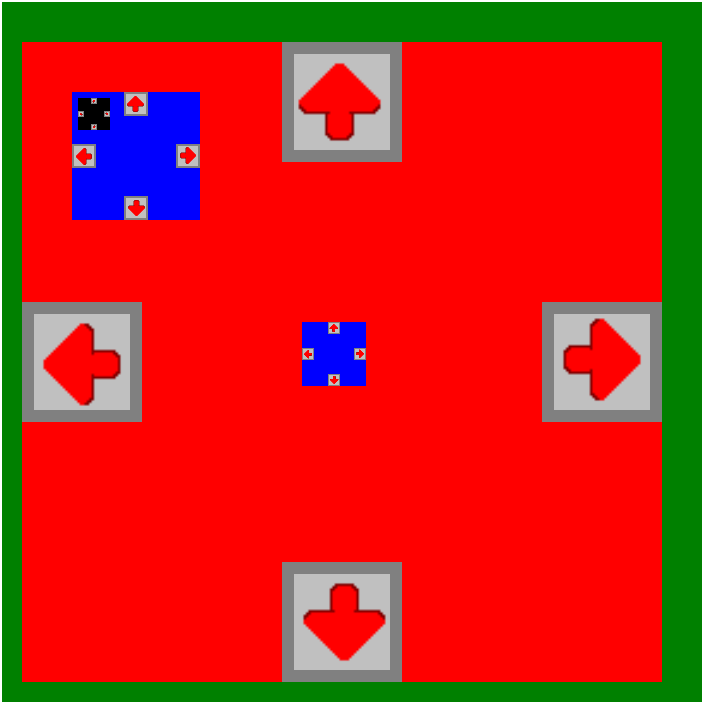
\includegraphics[width=\imglength]{GuiImg}%
	\vspace{-2\ht0}%
\end{wrapfigure}% 

%though 42 represents field accesses as method calls, for a fair comparison with conventional OO approach, we do not treat field accesses on \Q@SafeMovable@s within the \Q@SafeMovable@ class itself as public method calls
% D and Eiffel have slightly different interpretation of
% visible state semantic when qualified/unqualified method calls or field accesses are performed.
% However, in our GUI example those corner cases are
% not relevant. To be sure, we implemented both of their strategies and obtained the same results.
When we ran our test case following the D approach, the \Q!invariant()! method was called $52,734,053$ times, whereas the Eiffel approach `only' called it $14,816,207$ times;%
\footnote{
This difference is caused by Eiffel treating getters specially, and skipping invariant checks when calling a getter.
Thus, even ignoring getter methods, the visible state semantic would still run 14 millions of invariant checks.
}
in comparison our invariant protocol only performed $77$ calls. The number of checks is exponential in the depth of the GUI: the invariant of a \Q@SafeMovable@ will call the \Q@width()@, \Q@height()@, \Q@left()@, and \Q@top()@ methods of its children, which may themselves be \Q@SafeMovable@s, and hence such calls may invoke further invariant checks. Note that \Q!width()! and \Q!height()! are simply getters for fields, whereas the other two are non-trivial \emph{methods}.
Concluding, we have shown that when an invariant check queries other objects with invariants the visible state semantics may cause an exponential explosion in the number of checks.

 % Since we only use \Q@this@ to perform method calls, the invariant is not recursively checked on \Q@this@, if it were we would get an infinite recursion.
% Note that 42 represents field accesses as method calls, this is similar to the Eiffel uniform access principle; but for a fair comparison with D we treat private accesses to them like field accesses.


% It can be surprising to see such extreme difference. We ran our example with less widgets, and our results suggest an exponential growth in the cost of the conventional approach. For example by removing 2 containers (and their 8 buttons) we get....
% We now explain how this exponential explosion happens:
% For the outer-most box to check its invariant, it needs to call methods \Q@left,top,height@ and \Q@with@ to all its contained widgets.
% If one of those widget has \Q@invariant()@, when such public method is called,
% its \Q@invariant()@ is checked (twice). This requires to call \Q@left,top,height@ and \Q@with@ to all its contained widgets, some of those may also have invariants.

% In literature there is attention to prevent method called from an invariant to call public methods on \Q@this@; it would cause the system to go in loop.
% However when calling methods on other objects is allowed, if those objects have invariant, this cause the aforementioned explosion. 

% Our example also shows that the restrictions of TM's and object capabilities's are flexible enough to encode interactive GUI programs, where widgets may circularly reference other widgets.
% In order to perform this case study, we had to first implemented a simple Gui Library in L42. This library uses object capabilities to draw the widgets on screen, as well as fetch and dispatch the events.
% The gui library abstract away all the details of drawing and events; the user code need only to provide concrete classes implementing the \Q@Widget@ interface.

\subheading{Spec\# Comparison}
We also encoded our example in Spec\#\footnote{We compiled Spec\# using the latest available source (from 19/9/2014).}; that relies on pack/unpack; also called inhale/exhale or the Boogie methodology.
In pack/unpack, an object's invariant is checked only by the explicit pack operations.
In order for this to be sound, some form of aliasing and/or mutation control is necessary. Spec\# uses a theorem prover, together with source code annotations.
Spec\# can be used for full static verification, but it conveniently allows invariant checks to be performed at runtime, whilst statically verifying aliasing, purity and other similar standard properties.
This allows us to closely compare our approach with Spec\#.

As the back-end of the L42 GUI library is written in Java, we did not port it to Spec\#, rather we just simulated it, and don't actually display a GUI in Spec\#.
We ran our code through the Spec\# verifier (powered by Boogie~\cite{DBLP:conf/fmco/BarnettCDJL05}), which only gave us $2$ warnings\footnote{We used \Q@assume@ statements, equivalent to Java's \Q@assert@, to dynamically check array bounds. %. and value presence.
This aligns the code with L42, which also performs such checks at runtime.}, because the invariant of \Q@SafeMovable@ was not known to hold at the end of its constructor and \Q@dispatch(e)@ method. Thus, like our system, Spec\# checks the invariant
at those two points at runtime. Thus the code is equivalently verified in both Spec\# and L42; in particular it performed exactly the same number ($77$) of runtime invariant checks.

While the same numbers of checks are performed, we do not have the same guarantee provided by our approach:  Spec\#/Boogie does not soundly handle the non-deterministic impact of I/O, thus 
it does not properly prevent us from writing unsound
invariants that may be non-deterministic.
We also encoded our GUI in Microsoft Code Contracts~\cite{DBLP:conf/sac/FahndrichBL10}, whose unsound heuristic also calls the invariant $77$ times. However Code Contract does not enforce the
encapsulation of \Q@children()@, thus this approach is even less sound than Spec\#.

% Assuming that Spec\#'s verifier is sound, this means that our code is equally verified in Spec\# and L42, providing a reasonable comparison.
% Both Spec\# and L42 did the same thing:
% they statically verify ownership/aliasing annotations,
% they check the admissibility/valididty of a the invariant code and finally 
% they perform sufficient runtime-checking of the invariant.
% We used the Boogie static checker to verify all the aliasing/ownership properties needed to
% ensure that the $77$ run-time invariant checks soundly enforce that the invariant holds when is expected.
% This of course includes preventing the Gui to ever display two overlapping Widget. 

%\end{itemize}
%The result is the same of L42: the invariant is checked $77$ times, and in exactly the same locations of L42.

Note how both our L42 and Spec\# code required us to use the box pattern for our \Q@SafeMovable@, due to the cyclic object graph caused by the \Q@Action@s of \Q@Button@s needing to change their enclosing \Q@SafeMovable@'s position.
We found it quite difficult to encode the GUI in Spec\#, due to its unintuitive and rigid ownership discipline. In particular we needed to use many more annotations, which were larger and had greater variety. The following table shows the annotation burden,
for the \emph{program} that defines and displays the \Q@SafeMovable@s and our GUI; as well as the \emph{library} which defines \Q@Button@s, \Q@Widget@, and event handling. We only count constructs Spec\# adds over C\# as annotations, we also do not count annotations related to array bounds or null checks:
\begin{center}\SS
\begin{tabular}{ c  c  c  c  c}
 & Spec\# & Spec\# & L42 & L42 \\ 
 & \!\!program & library & program & library \\
\hline
 
\!\!\!Total number of annotations 
 	& $40$ & $19$ & $19$ & $18$ \\ \hline
% Totals 	 $59$ $37
\!\!\!Tokens (except \Q@.,;(){}[]@ and whitespace)\!\!\!
%(ecluding \Q@;,@ characters, white-space, or parentheses/brackets.) 
	& $106$ & $34$ & $19$ & $18$  \\  \hline
% $140$  & $37$
Characters (with minimal whitespace) 
	& $619$ & $207$ & $74$ & $60$ \\ \hline
%  $826$ $134$
\end{tabular}
\end{center}
\lstset{morekeywords={requires}}

To encode the GUI example in L42, the only annotations we needed were the 3 reference capabilities: \Q@mut@, \Q@read@, and \Q@capsule@ (\Q!rep! fields in the actual L42 language use the \Q!capsule! keywords to minimise language complexity);
% , for a total of 
% $19$ annotations (one token each, $74$ characters in total).
Our Spec\# code requires purity, immutability, ownership, method pre/post-conditions and method modification annotations. In addition, it requires the use of 4 different ownership functions including explicit ownership assignments. In total we used 18 different kinds of annotations in Spec\#.
\IO[28.3]{}The table presents token and character counts to compare against Spec\#'s annotations, which can be quite long and involved, whereas ours are just single keywords.
Consider for example the Spec\# pre-condition on \Q@SafeMovable@'s constructor: \\
\indent\Q@requires Owner.Same(Owner.ElementProxy(children), children);@

% methods and field attributes as well as requires, ensures and modifies clauses, and finally also %explicit ownership assignment statements.
% Spec\# annotation can be involved, as for example \Q@requires Owner.Same(Owner.ElementProxy(children), children);@}

% To estimate the annotation burden we count the number of tokens (excluding \Q@.;,@ and parenthesis).
% This gave us $113$ tokens, that is more then $5$ times the amount needed in L42.
% The total annotation character count is $830$; $10$ times more then L42.


% 40   106+17=113 619+211
%main 11 annotations, 28 + 11 tokens, 118+65 characters
%safemovable 29 annotations, 78+6 tokens, 501+146 characters

%19   34   207+44
% auxLib // 14 annotations, 25 tokens, 155+44 characters
%guiLib// 5 annoations, 9 tokens, 52 characters

% Moreover, in L42 we only use $3$ different kinds of annotations, while in Spec\# we use $15$ kinds of annotations.

\noindent The Spec\# code also required us to deviate from the code style shown in our simplified version: we could not write a usable \Q@children()@ method in \Q@Widget@ that returns a list of children, instead we had to write \Q@children_count()@ and \Q@children(int i)@ methods; we also needed to create a trivial class with a \Q@[Pure]@ constructor (since \Q@Object@'s one is not marked as such). In contrast, the only indirection we had to do in L42 was creating \Q@Box@es by using 
an additional variable in a nested scope.
This is needed to delineate scopes for promotions.
Based on these results, we believe our system is significantly simpler and easier to use
in comparision with Spec\#, that is more verbose but supports a wider range of verification applications.
% On the basis of these results we believe  that our system is easier to use for programmers that are not experts in software verification.

